% Template para o relatório final de estágio
% Autor: Fábio Engel de camargo

\documentclass{config/utfpr-style-estagio}
%%%% variaveis.tex, 2022/05/02, 2.4a
%%%% Copyright (C) 2020 Vinicius Pegorini (vinicius@utfpr.edu.br)
%%
%% This work may be distributed and/or modified under the conditions of the
%% LaTeX Project Public License, either version 1.3 of this license or (at your
%% option) any later version.
%% The latest version of this license is in
%%   http://www.latex-project.org/lppl.txt
%% and version 1.3 or later is part of all distributions of LaTeX version
%% 2005/12/01 or later.
%%
%% This work has the LPPL maintenance status `maintained'.
%%
%% The Current Maintainer of this work is Vinicius Pegorini.
%% Updated by:
%% - Marco Aurélio Graciotto Silva;
%% - Rogério Aparecido Gonçalves;
%% - Luiz Arthur Feitosa dos Santos.
%%
%% This work consists of the files utfpr.cls, main.tex, and
%% variaveis.tex.
%%
%% A brief description of this work is in readme.txt.

%% ####################################################
%%
%% >> Atenção - Leia isso antes de usar esse template<< 
%%
%% Esse template foi desenvolvido por professores,  com a intenção de ajudar os alunos com as entregas na biblioteca. Não há uma equipe especializada e dedicada mantendo tal template, mas sim professores trabalhando além das suas funções básicas, que são: ensino, pesquisa e extensão.
%
%% Também os mantenedores deste template não são especializados em LaTeX, muito menos em normas da ABNT. Todos que contribuíram com o template fizeram isso visando deixá-lo o mais próximo possível das normas da ABNT e das regras, anseios e expectativas da biblioteca da UTFPR. É muito importante entender que os desenvolvedores do template não têm relação direta com a biblioteca ou com a ABNT. Ou seja, não são os desenvolvedores do template que ditam as regras e normas dos textos que devem ser entregues à biblioteca.

%%É válido informar também, que como não há uma equipe dedicada e especializada, o tempo para colaborar com o template é curto. Desta forma, pode ser que não sejam empregadas as melhores técnicas, métodos e ferramentas para o desenvolvimento do template. Também pode acontecer do template não atender completamente todos os anseios e exigências da ABNT e da biblioteca, pois por exemplo, muitas regras de redação possuem questões interpretativas. Assim, o template sempre estará em contínua evolução e seria extremamente interessante que as pessoas (alunos,  professores,  técnicos e entusiastas) colaborarem com a evolução do template. Toda ajuda será bem vinda! Isso pode ser feito enviando e-mail para os desenvolvedores, desta forma, assim que possível esses vão tentar melhorar o template.

%%O template é apenas mais uma ferramenta para o desenvolvimento de trabalhos para a biblioteca. Todavia, podem existir outros templates LaTeX. Assim como há templates em outros formatos, que não o LaTeX. O mais importante é que qualquer pessoa, utilizando a princípio qualquer ferramenta, pode desenvolver textos que atendem os requisitos da biblioteca apenas estudando, interpretando e seguindo as regras da UTFPR e da ABNT, que estão disponíveis na página Web da instituição. O template é só um facilitador.

%%Por fim,  é necessário entender que infelizmente o ambiente LaTeX pode ser complexo e gerar resultados distintos dependendo do: sistema operacional,  pacotes LaTeX utilizados,  configurações alteradas, editor utilizado, a forma que está sendo redigida textos, figuras,  etc. Assim não há como garantir que o resultado final será o esperado.  Dito tudo isso,  >>UTILIZE ESSE TEMPLATE POR SUA CONTA E RISCO<<. Os desenvolvedores e colaboradores deste template não se responsabilizam pelo resultado do uso deste template e se eximem de qualquer responsabilidade.

%###################################################

%% Documento
%% Luiz: Define a fonte do texto da monografia
\fonteTexto{\sfdefault} % utilize \rmdefault para Times New Roman ou \sfdefault para Arial
\TipoDeDocumento{Trabalho de Conclusão de Curso de Graduação}%% Tipo de documento: "Tese", "Dissertação" ou "Trabalho de Conclusão de Curso de Graduação", "Estágio Supervisionado"
\NivelDeFormacao{Bacharelado}%% Nível de formação: "Doutorado", "Mestrado", "Bacharelado" ou "Tecnólogo" - ATENÇÃO, isso será utilizado para alterar a formatação do trabalho, pois pode haver formatações distintas dependendo o nível/tipo de trabalho.


%% luiz
% Template LaTex criado pelo Departamento Acadêmico de Computação (DACOM)
% da Universidade Tecnológica Federal do Paraná - Campus Campo Mourão (UTFPR-CM)
% Criado e alterado pelos professores:
% - Marco Aurélio Graciotto Silva
% - Rogério Aparecido Gonçalvez
% - Luiz Arthur Feitosa dos Santos
% Esse template utiliza a licença CC BY:
% Esta licença permite que outros distribuam, remixem, adaptem e criem a partir deste trabalho, mesmo para fins comerciais, desde que atribuam o devido crédito pela criação original.
% https://creativecommons.org/licenses/by/4.0/deed.pt_BR

% Dados do curso. Caso seja BCC:
%\program{Curso de Bacharelado em Ciência da Computação}
%\programen{Undergradute Program in Computer Science}
%\degree{Bacharel}
%\degreearea{Ciência da Computação}
 %Caso seja TSI:
\program{Curso Superior de Tecnologia em Sistemas para Internet}
\programen{Undergradute Program in Tecnology for Internet Systems}
\degree{Tecnólogo}
\degreearea{Tecnologia em Sistemas para Internet}


% Dados da disciplina. Escolha uma das opções e a descomente:
% TCC1:
%\goal{Proposta de Trabalho de Conclusão de Curso de Graduação}
%\course{Trabalho de Conclusão de Curso 1}
% TCC2:
 \goal{Trabalho de Conclusão de Curso de Graduação}
 \course{Trabalho de Conclusão de Curso 2}


% Dados do TCC (precisa alterar)
\author{Coloque o nome completo do(a) autor(a) aqui}  % Seu nome
\authorbib{Silva, João da} % Seu nome para referência bibliográfica (Sobrenome, Nome)
\title{Coloque o título aqui - O título deve ser claro e preciso} % Título do trabalho
\titleen{Put your english title here} % Título traduzido para inglês
\advisor{Prof. Dr. Fábio Engel de Camargo} % Nome do orientador. Lembre-se de prefixar com "Prof. Dr.", "Profª. Drª.", "Prof. Me." ou "Profª. Me."}
% Se não houver corientador, comente a linha a baixo
%\coadvisor{Nome Orientador completo e título} % Nome do coorientador, caso exista. Caso não exista, comente a linha.
\depositshortdate{2025} % Ano em que depositou este documento
\approvaldate{01/julho/2025}

% Dados do curso que não precisam de alteração
\university{Universidade Tecnológica Federal do Paraná}
\universityen{Federal University of Technology -- Paraná}
\universitycampus{Campus Campo Mourão}
\universityunit{Departamento Acadêmico de Computação}
\address{CIDADE}
\addressen{Campo Mourão, PR, Brazil}
\documenttype{Monografia}
\documenttypeen{Monograph}
\degreetype{Graduação}

\evalboardmember{Nome completo e por extenso do Membro 1}{Título (especialização, mestrado, doutorado}{Nome completo e por extenso da instituição a qual possui vínculo}
\evalboardmember{Nome completo e por extenso do Membro 2}{Título (especialização, mestrado, doutorado}{Nome completo e por extenso da instituição a qual possui vínculo}
\evalboardmember{Nome completo e por extenso do Membro 3}{Título (especialização, mestrado, doutorado}{Nome completo e por extenso da instituição a qual possui vínculo}
\evalboardmember{Nome completo e por extenso do Membro 4}{Título (especialização, mestrado, doutorado}{Nome completo e por extenso da instituição a qual possui vínculo}

%% Palavras-chave e keywords
%% ATENÇÃO - você deve indicar a quantidade de palavras chaves para o template LaTeX utilizar o pontuação correta!
\NumeroDePalavrasChave{5}%% Número de palavras-chave (máximo 5)
%% Atenção - por enquanto o template não está suportando acentos normais na palavra chave, por isso caso a palavra tenha acento, você deve utilizar o estilo antigo do LaTeX, sendo os acentos: á - \'a  é - \'e   â - \^a  ê - \^e  à - \`a  ä - \"a  ç - \c{c}
\PalavraChaveA{Palavra-chave 1}%% Palavra-chave A
\PalavraChaveB{Palavra-chave 2}%% Palavra-chave B
\PalavraChaveC{Palavra-chave 3}%% Palavra-chave C
\PalavraChaveD{Palavra-chave 4}%% Palavra-chave D
\PalavraChaveE{Palavra-chave 5}%% Palavra-chave E
%% Exemplo de como utilizar acentos na Palavra-chave:
% \PalavraChaveA{ol\'a}%% Olá
%\PalavraChaveB{voc\^e}%% você
%\PalavraChaveC{\`a}%% à
%\PalavraChaveD{a\c{c}\~ao}%% ação
%\PalavraChaveE{arg\"uir}%% argüir


%% ATENÇÃO - você deve indicar a quantidade de keywords para o template LaTeX utilizar o pontuação correta!
\NumeroDeKeywords{5}%% Número de keywords (máximo 5)
\KeywordA{Keyword 1}%% Keyword A
\KeywordB{Keyword 2}%% Keyword B
\KeywordC{Keyword 3}%% Keyword C
\KeywordD{Keyword 4}%% Keyword D
\KeywordE{Keyword 5}%% Keyword E


% É obrigatório o uso de uma licença Creative Commons (CC) nos trabalhos de TCC pelos cursos ligados a DACOM da UTFPR-CM.
% Veja: http://portal.utfpr.edu.br/biblioteca/trabalhos-academicos/docentes/procedimento-de-entrega-graduacao

% Sendo assim, escolha com o seu orientador uma das licenças CC a seguir: 

% CC BY: Esta licença permite que outros distribuam, remixem, adaptem e criem a partir deste trabalho, mesmo para fins comerciais, desde que atribuam o devido crédito pela criação original. Essa é a menos restritiva.
\licenca{ccby}

% CC BY CA: Esta licença permite que outros remixem, adaptem e criem a partir deste trabalho, mesmo para fins comerciais, desde que atribuam o devido crédito e que licenciem as novas criações sob termos idênticos.
%\licenca{ccbysa}

% CC BY ND: Esta licença permite a redistribuição, comercial e não comercial, desde que o trabalho seja distribuído inalterado e no seu todo, com crédito ao autor.
%\licenca{ccbynd}

% CC BY NC: Esta licença permite que outros remixem, adaptem e criem a partir deste trabalho para fins não comerciais, e embora os novos trabalhos tenham de atribuir o devido crédito e não possam ser usados para fins comerciais, os trabalhos derivados não têm que serem licenciados sob os mesmos termos.
%\licenca{ccbync}

% CC BY NC SA: Esta licença permite que outros remixem, adaptem e criem a partir deste trabalho para fins não comerciais, desde que atribuam ao autor o devido crédito e que licenciem as novas criações sob termos idênticos.
%\licenca{ccbyncsa}

% CC BY NC ND: Esta licença só permite que outros façam download do trabalho e o compartilhe desde que atribuam crédito ao autor, mas sem que possam alterá-los de nenhuma forma ou utilizá-los para fins comerciais. Essa é a mais restritiva.
%\licenca{ccbyncnd}

% Deixar sem licença - isso é aplicado apenas aos trabalhos que não são obrigados a ter licença. Na duvida verifique isso com o seu orientador e professor responsável pelo TCC. Para deixar o texto sem licença deixe o comando licença em brando ou deixe comentado.
%\licenca{}
% by DACOM/UTFPR-CM

\begin{document}
	\pretexto
	% define estilo do corpo do documento (capítulos e apêndices)
	\mainmatter
	\pagestyle{mainmatter}
	\chapter{Introdução}
\label{cap:introducao}
%=====================================================

Este Relatório de Estágio.....

\section{Exemplo de figura}

\begin{figure}[ht]
	\centering
	\caption{Exemplo de figura.}
	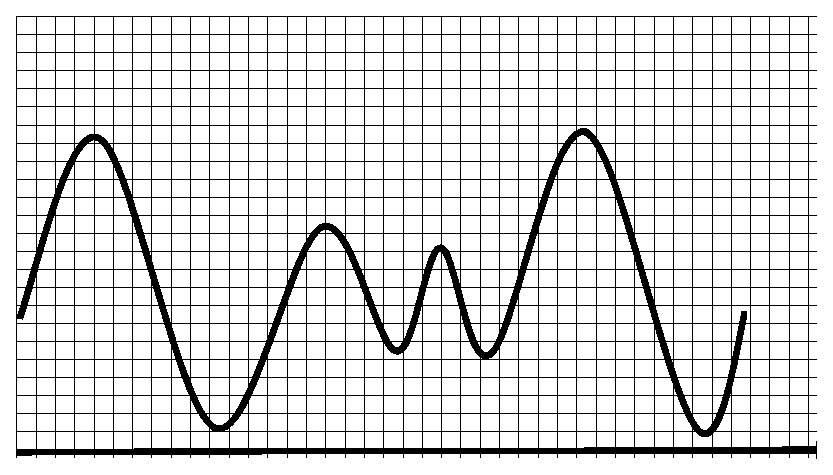
\includegraphics[width=0.5\textwidth]{fig/figexemplo.eps}
	\label{fig:figexemplo}
\end{figure}


\section{Exemplo de tabela}

\begin{table}[ht]
	\centering
	\caption{Exemplo de tabela.}
	\label{tab:exemplo}
	\begin{tabular}{|c|c|c|}
		\hline
		\textbf{Coluna 1} & \textbf{Coluna 2} & \textbf{Coluna 3} \\ \hline
		Linha 1 & Valor 1 & Valor 2 \\ \hline
		Linha 2 & Valor 3 & Valor 4 \\ \hline
	\end{tabular}
\end{table}

\section{Exemplos de citações}

Nesta seção são apresentados alguns exemplos de como realizar citações. Note que podem ser utilizados as macros \verb|\citet| e \verb|\cite|. A macro \verb|\citet| é utilizada para citar referências no formato de texto normal, em que o nome do autor (ou autores) e o ano da publicação são apresentados no texto. A macro \verb|\cite| é utilizada para citar referências entre parênteses, em que o nome do autor (ou autores) e o ano da publicação são apresentados dentro dos parênteses.

\subsection{Exemplo 1}
Neste ano, o Núcleo de Informação e Coordenação do Ponto BR (NIC.br), responsável pela administração e coordenação do domínio de topo ``.br'' da Internet, emitiu um alerta sobre a iminente escassez de endereços IPv4. Em 31 de janeiro, os últimos blocos disponíveis de endereços IPv4 foram distribuídos, incluindo para a região da América Latina e Caribe, da qual o Brasil faz parte. Estima-se que o Brasil ainda possua estoque de endereços IPv4 no padrão ``.br'' para distribuição por mais um ano, por meio do NIC.br \citep{nicbr2023IANA}.

\subsection{Exemplo 2}
O estudo de \citet{spanhol2015dataset} apresenta um conjunto de dados composto por 7.909 imagens de histopatologia de câncer de mama, obtidas de 82 pacientes, e disponíveis em uma plataforma pública. O conjunto de dados, disponibilizado em \url{http://web.inf.ufpr.br/vri/breast-cancer-database}, inclui imagens tanto benignas quanto malignas e é destinado à tarefa de classificação automatizada dessas imagens em duas classes. Essa ferramenta de diagnóstico auxiliado por computador pode ser valiosa para os clínicos. 

\subsection{Exemplo 3}

A utilização da lógica fuzzy combinada a técnicas analíticas pode ser uma abordagem eficaz para alcançar maior eficiência energética em dispositivos de redes de sensores sem fios (\textit{Wireless Sensor Networks} - WSNs). Essa abordagem propõe o uso de métodos eficientes de seleção de retransmissores para melhorar a vida útil da bateria, o desempenho e a eficiência energética das WSNs \cite{engel2013relay}.

\subsection{Exemplo 4}

Nos dias atuais, as tecnologias modernas de tecnologia da informação têm sido amplamente utilizadas com o objetivo de aprimorar a eficiência e o desempenho de sistemas de produção e de rede. Essas tecnologias, como Internet das Coisas (IoT), Redes de Funções Virtuais (NFV), Aprendizado de Máquina e outras, têm sido aplicadas em diversos contextos, desde manufatura aditiva (impressão 3D) até gerenciamento de redes de telecomunicações. Essas abordagens inovadoras visam obter ganhos significativos em termos de otimização de processos, monitoramento em tempo real, detecção de falhas, automação e tomada de decisões baseada em dados \cite{huff2020building,scheffel2021automated}. 


	\chapter{Do Local de Estágio}
\label{cap:localestagio}
%=====================================================

Descrever a empresa onde o estágio foi desenvolvido.
	\chapter{Do Plano De Estágio}
\label{cap:plano}
%=====================================================

Descrever o plano de estágio, as atividades definidas e os prazos estipulados.
	\chapter{Descrição e Análise das Atividades Desenvolvidas}
\label{cap:descricao}
%=====================================================

Neste capítulo o estagiário fala detalhadamente das atividades que desenvolveu ao longo do estágio, sendo fundamental que estabeleça a relação entre a teoria e a prática. Caso tenha feito estágio em mais de uma área, pode-se dividir este capítulo em subtítulos. 
O desenvolvimento é a parte principal e mais extensa, que contém a exposição ordenada e pormenorizada do assunto, onde o estagiário apresenta as atividades desenvolvidas durante o estágio. Podem ser colocados desenhos, fotografias, gráficos, mapas, organogramas, fluxogramas, quadros, tabelas e figuras para melhor ilustração e comprovação das atividades desenvolvidas.

	\chapter{Conclusão}
\label{cap:conclusao}
%=====================================================

Concluir o relatório com uma pequena retomada das principais atividades desenvolvidas analisando a respectiva contribuição à sua formação profissional. Os pontos fortes e fracos do estágio.
	\chapter{Considerações Finais}
\label{cap:consideracoes}
%=====================================================

Esta é a parte final do Relatório de Estágio, na qual o estagiário deve apresentar as últimas considerações sobre seu estágio supervisionado.  % Este é opcional. Comentar, caso não deseje utilizar.
	
	%Só se coloca este item caso o estagiário tenha citado algum trecho de livro, apostila, artigo da Internet, enfim, qualquer item  publicado ou de acesso livre ao público em geral.
	\bibliography{bibliografia}
	
	%items opcionais. Comentar caso não utilize.
	\chapter{Apêndice}
\label{cap:apendice}

Neste capítulo colocam-se os itens criados pelo próprio estagiário, como por exemplo, uma ficha de cadastro de clientes, um programa de computador, um roteiro de entrevista, enfim, qualquer elemento criado pelo estagiário. Este capítulo não é obrigatório, desde que o estagiário não mencione no decorrer do seu relatório algo que ele tenha criado ou elaborado para a empresa concedente do estágio. Elemento opcional. 
É o texto ou documento com a finalidade de complementar sua argumentação, sem prejudicar o sentido do trabalho. O apêndice é identificado por letras maiúsculas consecutivas, travessão e pelos respectivos títulos. Excepcionalmente, utilizam-se letras maiúsculas dobradas, na identificação dos apêndices, quando esgotadas as letras do alfabeto.
	\chapter{Anexos}
\label{cap:anexos}

Elemento opcional, sendo um texto ou documento não elaborado pelo autor, que serve de fundamentação, comprovação e ilustração. Os anexos são identificados por letras maiúsculas consecutivas, travessão e pelos respectivos títulos. Excepcionalmente, utilizam-se letras maiúsculas dobradas, na identificação dos anexos, quando esgotadas as 26 letras do alfabeto.
\end{document}
